% generated by scripts/pkl_to_latex.py
% source PKL : vscan_v1_L6_Ne6_U10_t1_mode-uniform_nmin2_solver-gcg_full_restarts8_iter300_kmax4_tol1em09_V0to15_N16-2f7c06936fa2.pkl
% scan type  : vscan
% state      : gs
% requires   : \usepackage{pgfplots} \pgfplotsset{compat=1.18}
% colours match the matplotlib PDF (tab10 cycle)
\definecolor{gmeC0}{HTML}{1F77B4}
\definecolor{gmeC1}{HTML}{FF7F0E}
\definecolor{gmeC2}{HTML}{2CA02C}
\definecolor{gmeC3}{HTML}{D62728}
\definecolor{gmeC4}{HTML}{9467BD}
\definecolor{gmeC5}{HTML}{8C564B}
\definecolor{gmeC6}{HTML}{E377C2}
\definecolor{gmeC7}{HTML}{17BECF}

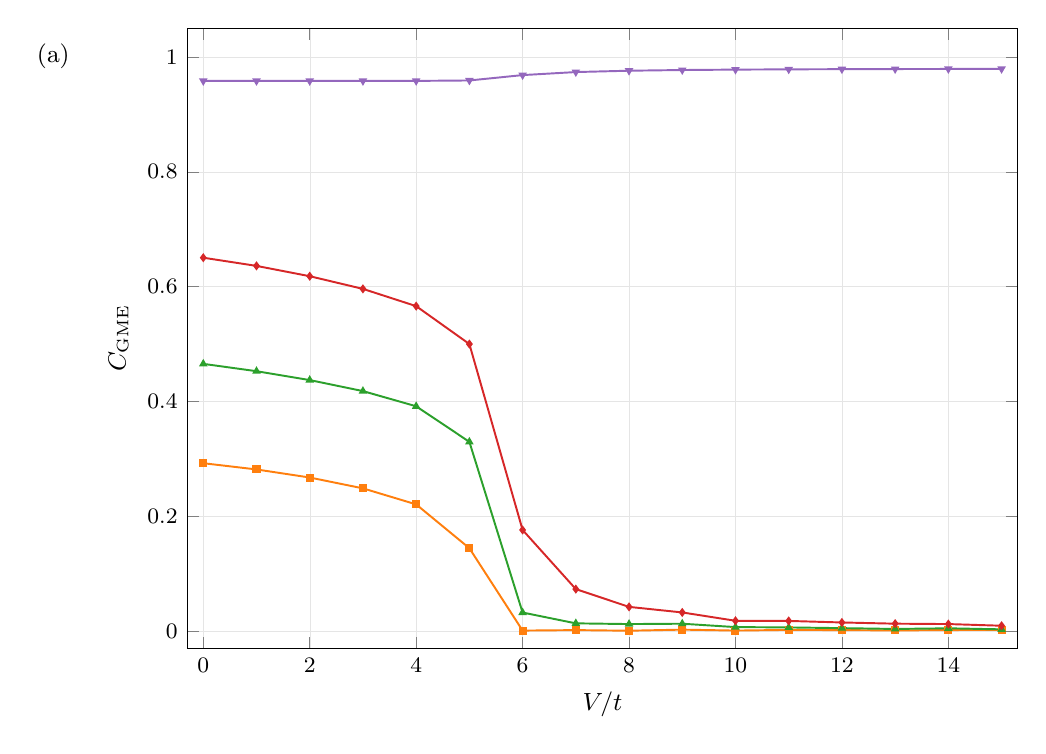
\begin{tikzpicture}
  \begin{axis}[
    width=\columnwidth,
    height=0.78\columnwidth,
    xlabel={$V/t$},
    ylabel={$C_{\mathrm{GME}}$},
    grid=both,
    grid style={line width=.1pt, draw=gray!20},
    tick label style={font=\footnotesize\rmfamily, /pgf/number format/fixed},
    label style={font=\small\rmfamily},
    scaled ticks=false,
    legend style={font=\scriptsize\rmfamily, draw=gray!40, at={(0.5,1.03)}, anchor=south, /tikz/every even column/.append style={column sep=6pt}},
    legend cell align={left},
    legend columns=2,
    ymin=-0.03,
    ymax=1.05,
    xmin=-0.3,
    xmax=15.3,
    after end axis/.append code={\node[anchor=east, font=\small\rmfamily] at (axis description cs:-0.13,0.954) {(a)};},
  ]
    \addplot[color=gmeC1, mark=square*, mark size=1.1pt, line width=0.7pt] coordinates {
        (0,0.292503) (1,0.281631) (2,0.267581) (3,0.248713)
        (4,0.220801) (5,0.144459) (6,0.001014) (7,0.001859)
        (8,0.000778) (9,0.002676) (10,0.001031) (11,0.00221)
        (12,0.001859) (13,0.001286) (14,0.001883) (15,0.002424)
    };
    \addplot[color=gmeC2, mark=triangle*, mark size=1.1pt, line width=0.7pt] coordinates {
        (0,0.46551) (1,0.452726) (2,0.437276) (3,0.418075)
        (4,0.391641) (5,0.32967) (6,0.032476) (7,0.013612)
        (8,0.012382) (9,0.012989) (10,0.007099) (11,0.006528)
        (12,0.005277) (13,0.00386) (14,0.004993) (15,0.003191)
    };
    \addplot[color=gmeC3, mark=diamond*, mark size=1.1pt, line width=0.7pt] coordinates {
        (0,0.65035) (1,0.636103) (2,0.618138) (3,0.596071)
        (4,0.566042) (5,0.50003) (6,0.176248) (7,0.073264)
        (8,0.042297) (9,0.032611) (10,0.018109) (11,0.017831)
        (12,0.015149) (13,0.013052) (14,0.012387) (15,0.009468)
    };
    \addplot[color=gmeC4, mark=triangle*, mark size=1.1pt, mark options={rotate=180}, line width=0.7pt] coordinates {
        (0,0.958182) (1,0.958185) (2,0.958191) (3,0.958207)
        (4,0.958267) (5,0.95901) (6,0.968364) (7,0.973662)
        (8,0.975992) (9,0.977209) (10,0.977923) (11,0.978378)
        (12,0.978685) (13,0.978903) (14,0.979062) (15,0.979182)
    };
  \end{axis}
\end{tikzpicture}
